%%%%%%%%%%%%%%%%%%%%%%%%%%%%%%%%%%%%%%%%%%%%%%%%%%%%%%%%%%%%%%%%%%%%%
% U.S. ELT KEY SCIENCE PROGRAM DESCRIPTION DOCUMENT ("PROPOSAL")
% Version 1.3, 1 November 2018
%%%%%%%%%%%%%%%%%%%%%%%%%%%%%%%%%%%%%%%%%%%%%%%%%%%%%%%%%%%%%%%%%%%%%

% LaTeX template for writing US ELT Program Key Science Program Description Documents
% (aka "proposals").
% 
% Please fill in all sections.
% 
% The Scientific Justification should be limited to 4 pages including figures (but not including
% references.) There are no strict page limits for other sections, or for the documen
t as a whole, 
% but we suggest a guideline of 8 to 10 pages (excluding cover page and investigators) for the 
% whole document.

%%%%%%%%%%%%%%%%%%%%%%%%%%%%%%%%%%%%%%%%%%%%%%%%%%%%%%%%%%%%%%%%%%%%%

% Please do not modify or delete the following lines.
\documentclass[11pt]{article}
\usepackage{useltp_ksp_1.3}
\usepackage{deluxetable}
\usepackage{natbib}
\begin{document}
\bibliographystyle{aasjournal}

%%%%%%%%%%%%%%%%%%%%%%%%%%%%%%%%%%%%%%%%%%%%%%%%%%%%%%%%%%%%%%%%%%%%%

% SCIENTIFIC CATEGORIES
%
% Please select a scientific category that best describes your
% program by uncommenting only ONE of the selections below.  
% NOTE:  We will probably change this in a future update to allow
% multiple topical areas.

% \sciencecategory{Our Solar System}
% \sciencecategory{Extra-Solar Planetary Systems}
% \sciencecategory{Star and Planet Formation}
% \sciencecategory{Stars and Stellar Evolution}
% \sciencecategory{Resolved Stellar Populations and their Environments}
% \sciencecategory{Galaxy Evolution}
% \sciencecategory{Cosmology and Fundamental Physics}
% \sciencecategory{Astronomical Transients and Multi-Messenger Astrophysics}

%%%%%%%%%%%%%%%%%%%%%%%%%%%%%%%%%%%%%%%%%%%%%%%%%%%%%%%%%%%%%%%%%%%%%%

% TITLE
%
% Give a descriptive title for the proposal in the \title{} command.
%
% Note that a title can be quite long; LaTeX will break the title into
% separate lines automatically.  If you wish to indicate line breaks
% yourself, do so with a `\\' command at the appropriate point in
% the title text.  Use both upper and lower case letters (NOT ALL CAPS).

\title{The Birth and Death of Stars: Initial and Final Mass Functions}

%%%%%%%%%%%%%%%%%%%%%%%%%%%%%%%%%%%%%%%%%%%%%%%%%%%%%%%%%%%%%%%%%%%%%%

% ABSTRACT
%
% Give a general abstract of the scientific justification appropriate
% for a non-specialist.  Write between the \begin{abstract} and 
% \end{abstract} lines.  

% DO NOT remove the \begin{abstract} and \end{abstract} lines.

\begin{abstract}
While the bulk of stellar evolution is broadly understood, there are two key phases where we have gaping holes in our knowledge: star birth and death. 
At the formation stage, we still lack a predictive model of star
%MA2: and BD 
formation that can tell us the number and mass of stars that form (i.e. the initial mass function, IMF) from a given molecular cloud. At stellar death, we also lack a predictive model for %MA2 if and 
how a star of a
given mass explodes and what kind of remnant it leaves behind (i.e. the initial-final mass relation, IFMR). 
We propose a comprehensive study of both the birth and death
phase of stars through (1) measurements of the IMF as a function of
environment using direct star counts of a wide array of young star clusters and dwarf galaxies and (2) measurements of the IFMR of black holes, neutron stars, and white dwarfs using astrometric gravitational lensing. 
These studies are only possible with the increased spatial resolution of
the US-ELTs and visibility in both hemispheres in order
cover the full range of environments. 
\end{abstract}

%%%%%%%%%%%%%%%%%%%%%%%%%%%%%%%%%%%%%%%%%%%%%%%%%%%%%%%%%%%%%%%%%%%%%%

% TEAM MEMBER INFORMATION BLOCKS 
%
% Please give names, affiliations, and e-mail addresses of team members here.

% DO NOT remove the \teammembers, \begin{team_member} and \end{team_member} tags.  
% Only one individual's name per \name field is allowed.

\teammembers

\begin{team_member}
\name{Jessica R. Lu}
\affil{UC Berkeley}
\email{jlu.astro@berkeley.edu}
\end{team_member}

\begin{team_member}
\name{Matthew Hosek Jr.}
\affil{UCLA}
\email{mwhosek@astro.ucla.edu}
\end{team_member}

\begin{team_member}
\name{Rachel Beaton}
\affil{}
\email{}
\end{team_member}

\begin{team_member}
\name{Tuan Do}
\affil{UCLA}
\email{tdo@astro.ucla.edu}
\end{team_member}

\begin{team_member}
\name{Dongwon Kim}
\affil{UC Berkeley}
\email{dongwon.kim@berkeley.edu}
\end{team_member}

\begin{team_member}
\name{Evan Kirby}
\affil{Caltech}
\email{enk@astro.caltech.edu}
\end{team_member}

\begin{team_member}
\name{Michael Meyer}
\affil{University of Michigan}
\email{mrmeyer@umich.edu}
\end{team_member}

\begin{team_member}
\name{Morten Andersen}
\affil{Gemini Observatory}
\email{manderse@gemini.edu}
\end{team_member}

\begin{team_member}
\name{Sukanya Chakrabarti}
\affil{RIT}
\email{chakrabarti@astro.rit.edu}
\end{team_member}

\begin{team_member}
\name{Michael Medford}
\affil{UC Berkeley}
\email{}
\end{team_member}

\begin{team_member}
\name{Jennifer Sobeck}
\affil{UW}
\email{jsobeck@uw.edu}
\end{team_member}

\begin{team_member}
\name{Siyao Jia}
\affil{UC Berkeley}
\email{}
\end{team_member}
\begin{team_member}

\name{Paolo Turri}
\affil{UC Berkeley}
\email{}
\end{team_member}

\begin{team_member}
\name{Fatima Abdurrahman}
\affil{UC Berkeley}
\email{}
\end{team_member}

\begin{team_member}
\name{Nicholas Z. Rui}
\affil{UC Berkeley}
\email{}
\end{team_member}

\begin{team_member}
\name{Peter Boyle}
\affil{UC Berkeley}
\email{}
\end{team_member}

\begin{team_member}
\name{Casey Y. Lam}
\affil{UC Berkeley}
\email{casey$\_$lam@berkeley.edu}
\end{team_member}


% Duplicate and uncomment the \begin{team_member} to \end{team_member} blocks
% if you have additional team members.   Comment or remove any unneeded blocks.

%%%%%%%%%%%%%%%%%%%%%%%%%%%%%%%%%%%%%%%%%%%%%%%%%%%%%%%%%%%%%%%%%%%%%%
% MAIN PROPOSAL BODY
%%%%%%%%%%%%%%%%%%%%%%%%%%%%%%%%%%%%%%%%%%%%%%%%%%%%%%%%%%%%%%%%%%%%%%

% In the following "essay question" sections, the delimiting pieces of
% markup (\justification, \expdesign, etc.) act as LaTeX \section*{}
% commands.  If the author wanted to have numbered subsections within
% any of these, LaTeX's \subsection could be used.
%
% DO NOT REDUCE THE FONT SIZE, and do not otherwise fiddle with the
% format to get more on a page.  We will reset any changes back to the
% default font.
%
% If you wish to use our "reference" environment, follow the following
% example (journal commands are compatible with AASTeX v4.0):
%
%\begin{references}
%\reference Armandroff \& Massey 1991 \aj, 102, 927.
%\reference Berkhuijsen \& Humphreys 1989 \aap, 214, 68.
%\reference Massey 1993 in Massive Stars: Their Lives in the 
% Interstellar Medium (Review), ed. J. P. Cassinelli and E. B. 
% Churchwell, p. 168.
%\reference Massey \& Armandroff 1999, in prep.
%\end{references}

% PDF figures may be included as follows:
%
% \begin{figure}
%  \begin{center}
%   \includegraphics[width=4.0cm]{sample.pdf}
%   \caption{Sample figure showing important results.}
%  \end{center}
% \end{figure}

%%%%%%%%%%%%%%%%%%%%%%%%%%%%%%%%%%%%%%%%%%%%%%%%%%%%%%%%%%%%%%%%%%%%%%
% PROPOSAL SECTIONS
%%%%%%%%%%%%%%%%%%%%%%%%%%%%%%%%%%%%%%%%%%%%%%%%%%%%%%%%%%%%%%%%%%%%%%

% SCIENTIFIC JUSTIFICATION
%
% Describe the scientific context for this Key Science Program, the specific research question(s)
% to be addressed, and the overall significance to astronomy.  The Scientific Justification 
% should be limited to 4 pages including figures.

\sciencejustification

We experience the Universe through the light of stars and they 
act as a "fundamental particle" for much of astrophysics. 
While the bulk of stellar evolution is broadly understood, there are two key phases where we have gaping holes in our knowledge: star birth and death.

At the formation stage, we still lack a predictive model of star formation that can tell us the number and mass of stars that form from a given molecular cloud.
Observations provide evidence that the outcome of the star formation
process -- the initial mass function (IMF) -- is fairly uniform in the
local solar neighborhood \citep{Bastian:2010} which covers a relatively small range of cluster conditions.  
However, there is now evidence that the IMF varies in more extreme environments such as in the Galactic Center \citep{Lu:2013,Hosek:2018b} the most massive elliptical galaxies \citep{vanDokkum:2010}, or the least luminous Milky Way satellites \citep{Geha:2013}.
Today, the non-standard IMF claims are debated and can't easily be improved on due to the 
%MA2 high stellar densities in these regions and the 
lack of spatial resolution and field of view with HST and even 8-10 m telescopes with adaptive optics and JWST.
Mapping variations of the IMF with environment from direct star counts is a major observational challenge for the next generation of large telescopes. 

At stellar death, we also lack a predictive model for how a star of a
given mass explodes and what kind of remnant, if any, it leaves behind. 
This initial-final mass relation (IMFR) depends on the detailed physics of
core evolution in the last few hours of a stars life and during the
supernovae explosion. 
This has led to an order-of-magnitude uncertainty in the simplest
term: the number of BHs in the Galaxy. Other statistics, such as the
BH binary fraction, mass function, and kick velocity distribution, are
so uncertain that it is difficult to interpret current LIGO
discoveries ({\bf }, "Putting LIGO discoveries in context"?}). Ultimately, we need to measure a large range of masses
for compact objects, which is now possible using gravitational microlensing when a dark lens passes in front of a background star. 
Large samples of candidate dark lenses will be identified with next generation photometric surveys, such as WFIRST and LSST; however, current facilities cannot  deliver precise astrometry for such a large sample size.

We propose a comprehensive US-ELT study of both the birth and death
phase of stars through measurements of the IMF as a function of
environment and the IFMR of black holes, neutron stars, and white
dwarfs (Figure \ref{fig:top_level}). 
These studies require the power of
diffraction-limited observations with the US-ELTs from both hemispheres in order
cover the full range of environments. 

\begin{figure}[h]
    \centering
    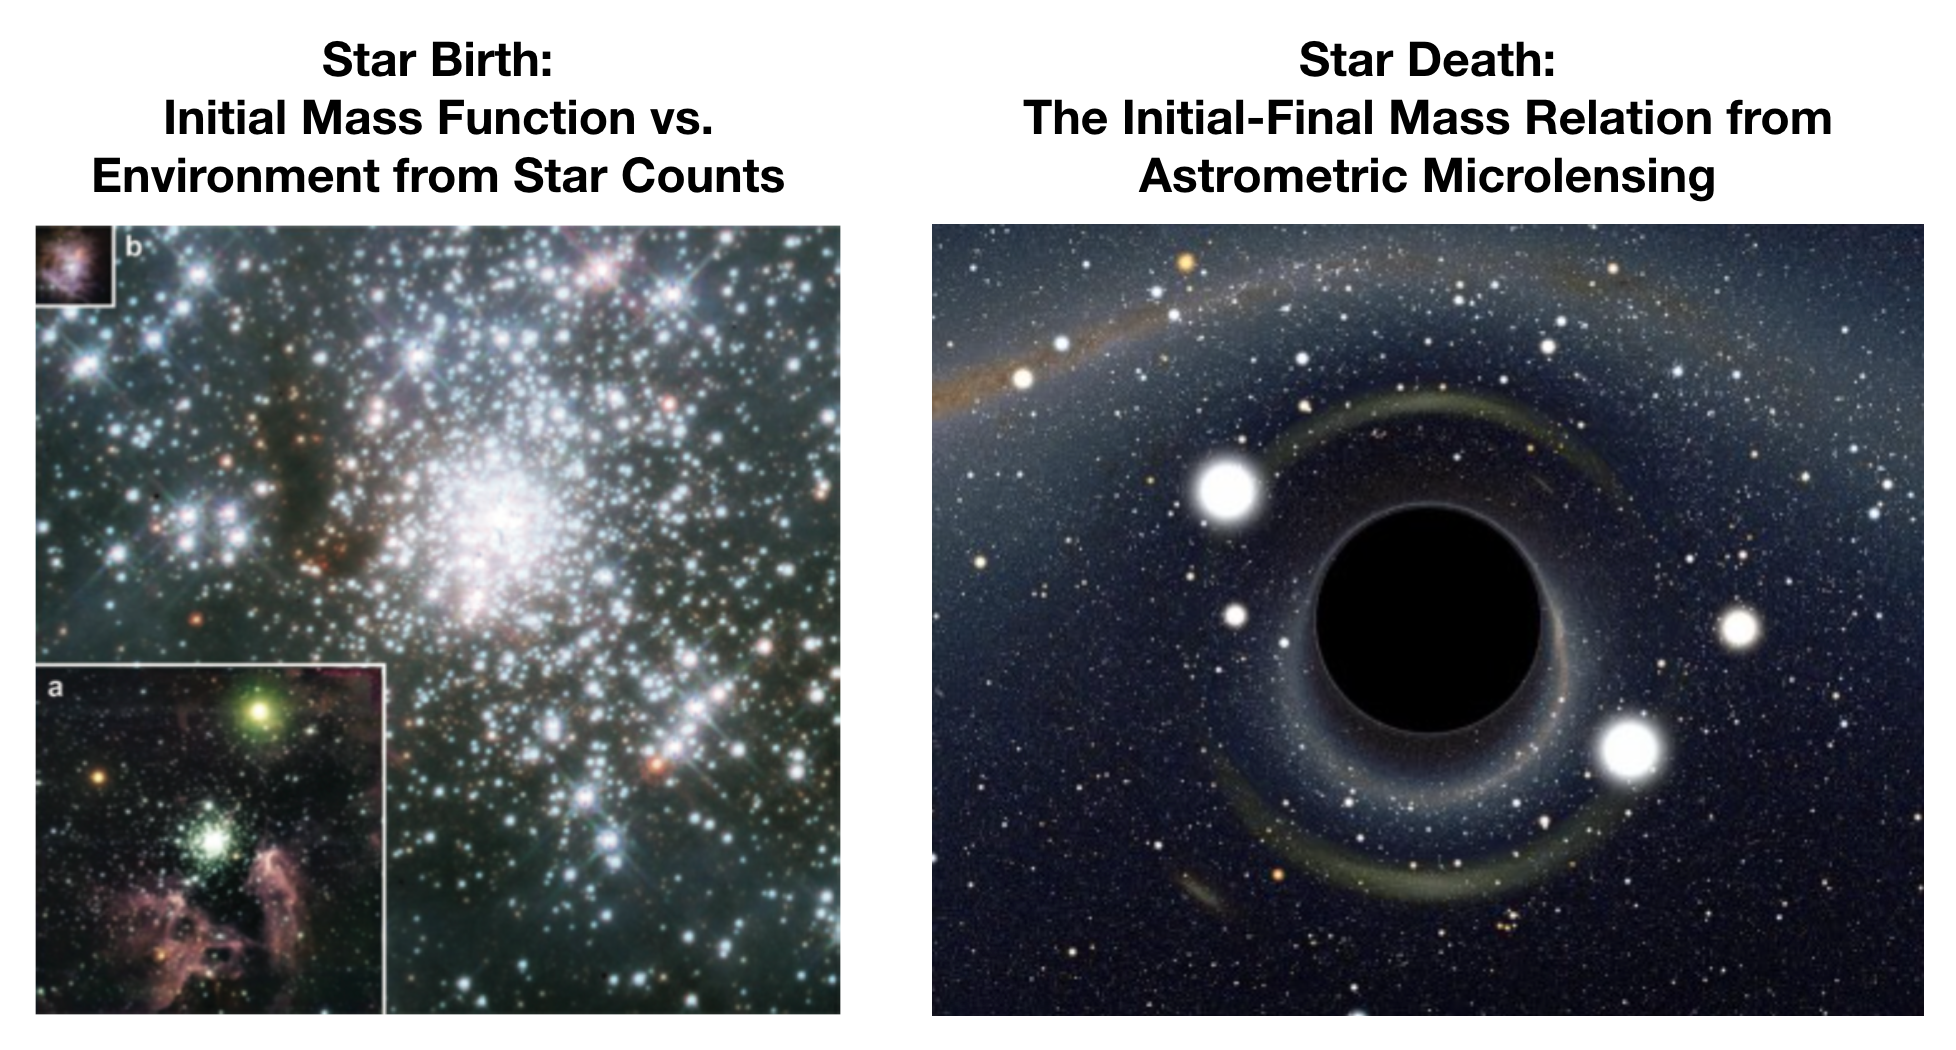
\includegraphics[scale=0.3]{ksp_useltp2018_fig1.png}
    \caption{{\em Left:} Young star clusters in different environments (metallicity, ambient pressure, density). Counting and weighing individual stars is the gold standard for deriving the IMF. Image reproduced from \citet{Zinnecker:2007}. {\em Right:} Black holes gravitationally lens background stars, allowing us to "see" and weigh them and ultimately constrain the IFMR.}
    \label{fig:top_level}
\end{figure}

{\bf \large The Initial Mass Function vs. Environment}

The quest for a predictive theory of star formation, as a function of initial conditions (metallicity, density, external pressure), is far from over.  
And almost as important (and frustratingly inseparable) are the properties of multiple systems (companion mass ratio distribution, surface density distribution, and frequency) as a function of primary star mass. 
Most observations reveal a “universal” IMF, and, not surprisingly, many diverse models are able to “explain” it. 
Under intense scrutiny, most claims of detecting a non-universal IMF wither \citep[c.f.][]{Bastian:2010,Luhman:2018}; however there are some unexplained surprises.  
Some of the most persistent, and puzzling, are the claims of bottom-heavy IMFs inferred from various techniques (population synthesis, dynamics, and strong lensing) toward giant elliptical galaxies \citep[e.g.][]{vanDokkum:2010}.  
In contrast, two massive young clusters at the Galactic Center appear to be top-heavy \citep{Lu:2013,Hosek:2018b}, and recent work points to a top-light IMF in the outskirts of an irregular dwarf galaxy \citep{2018MNRAS.477.5554W}. 
Unfortunately, nearby well-studied star forming regions are poor analogues for diverse star forming events at low metallicity, high pressure, and extreme density which may characterize environments in the early Universe, galactic nuclei, and merger events. 
%In order to fully understand the star formation process, the environments of planet formation in their midst, and to support models of galaxy formation and evolution, as well as the chemical evolution, and the frequency of stellar remnants (and stellar mergers) in the Universe over cosmic time, the sensitivity and angular resolution of ELTs is required.

Our objective is to measure the initial mass function from direct star counts from 150 M$_{\odot}$ stars down to brown dwarfs in a range of environments in the Milky Way and Local Group. The targets will include:
both massive and low-mass clusters (\bf{Jessica, low-mass corresponding to what mass? Much below ONC and it is a different approach observationally than the massive clusters}),
young star clusters in the Milky Way and M31 disk,
young star clusters in the Galactic and M31 center,
young star clusters in the low-metallicity LMC and SMC,
young star clusters in the closest starburst galaxies such as M82, and 
stars in low-metallicity dwarf galaxies.
These are generally crowded regions and the lowest-mass stars are extremely faint; thus, high spatial resolution and depth are essential (Table \ref{tab:cluster_props}). For example, resolved spectroscopic and imaging studies of young massive clusters near the Galactic Center are currently limited to the high-mass stars. In the era of ELTs, these limits are pushed well into the pre-main sequence (M $\lesssim$ 2.6 M$_{\odot}$)
%MA2 here and in the figure it would be good to point out what mass this is and in the figure to point to the main sequence and pre-main sequence parts of the isochrones. 
%mwhosek: I have updated the text and figure according to MA2 comment
for spectroscopy and well into the brown dwarf regime (M $\lesssim$ 0.07 M$_{\odot}$) for imaging (Figure \ref{fig:TMT_YNC})! In low density environments, the increased spatial resolution offered by ELTs will completely eliminate issues with star-galaxy separation, allowing IMFs to be estimated all the way down to the hydrogen limit for dozens of ultra-faint dwarf galaxies \citep{Gennaro+18a, Gennaro+18b}. In addition to revolutionizing our knowledge of the IMF for very low mass stars, %MA2 I think it should be stated strongly that unless we probe well past the peak of the IMF we won't learn too much; it's all scale free above 1 Msun with at best hints of flattening in the observations. 
these measurements will characterize the behavior of both the high-mass slope and turnover mass of the IMF, which are critically tied to the underlying physics driving star formation \citep{Offner:2014,Krumholz:2014}.

%MA2 Having the physical scales (and masses) for the clusters would help the non-expert reader appreciate the crowding problems as well as the difference in environments. 
%mwhosek: there might be something funny here about the Hydrogen burning limit mags. According to our GC isochrone, the hydrogen burning limit should be around Kp = 22.8 mag (the bottom of our isochrone).
\begin{deluxetable}{lccccc}
\tablewidth{0pt}
\tabletypesize{\footnotesize}
\tablecaption{Properties of Young Clusters in Different Environments \label{tab:cluster_props}}
\tablehead{
\colhead{Distance\tablenotemark{a}} & 
\colhead{Cluster Size} & 
\colhead{Stellar Separation} & 
\colhead{Proper Motion} & 
\colhead{Typical Binary} &
\colhead{Hydrogen Burning} \\
\colhead{} &
\colhead{} & 
\colhead{in Core} &
\colhead{for 10 km s$^{-1}$} &
\colhead{Separation} &
\colhead{Limit} \\
\colhead{(kpc)} & 
\colhead{(arcsec)} & 
\colhead{(arcsec)} & 
\colhead{(mas yr$^{-1}$)} & 
\colhead{(mas)} &
\colhead{(K mag)}
} 
\startdata
0.4 (Orion)           & 515.66 & 2.6 & 5.28 & 75.2 & 12.5 \\
8.0 (Galactic Center) & 25.78 & 0.13 & 0.264 & 3.76 & 19.0 \\
60 (LMC)              & 3.44 & 0.02 & 0.035 & 0.50 & 23.5 \\
3500 (M82)            & 0.06 & 3$\times 10^{-4}$ & $6\times 10^{-4}$ & $9\times 10^{-3}$ & 32.0 \\
\enddata
\vspace{-0.1in}
\tablenotetext{a}{Table modified from \citep{Lu:2009}. Cluster size is $\sim$1 pc in diameter. Star separations are based on ONC Trapezium and typical binary separations are $\sim$30 AU.}
\end{deluxetable}

Coupled with the measuring the IMF is understanding stellar multiplicity. In particular, the multiplicity fraction can be derived via spectroscopic monitoring, which can measure the doppler shifts induced by the orbital motion of the systems [CHECK REQUIRED RV PRECISIONS]. In addition, the gain in spatial resolution by a factor of 4 will enable us to resolve multiple stellar systems in star forming regions out to 2 kpc to the same detail as is obtained for the ONC today, and we can probe much more of the binary parameter space in the ONC and other nearby regions.
%MA2 We will also gain a factor of 4 in spatial resolution which will enable us to compare the 2kpc massive regions with present day ONC observations and will allow us to probe much more of binary parameter space in the ONC and other nearby regions. Both in terms of spatial resolution and contrast. 
%mwhosek: Isn't it only a gain of a factor of 3 in spatial resolution, going from a 10 -- 30 m telescope (assuming diffraction limited in both cases)? Regardless, I've added this text.
An exploration of multiplicity across different stellar environments has never been undertaken, and is only possible with ELTs. 

%mwhosek: ancillary science moved to legacy section

%Highlight: North (outer MW, M31) and South (MW, LMC/SMC for low-metallicity, 2 Mpc groups), and all sky (local group galaxies).
%MA Above we note that we can do IMF down to the BD limit at 100kpc, but need the limit at 2Mpc. :


\begin{figure}
    \centering
    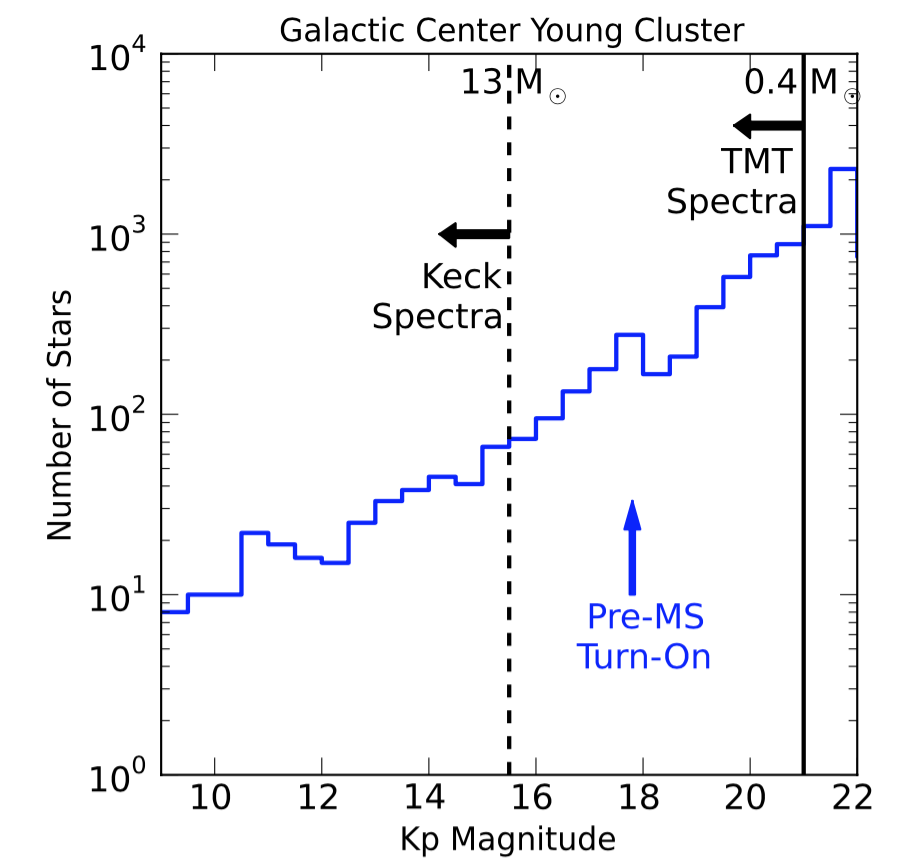
\includegraphics[scale=0.47]{TMT_YNC.png}
    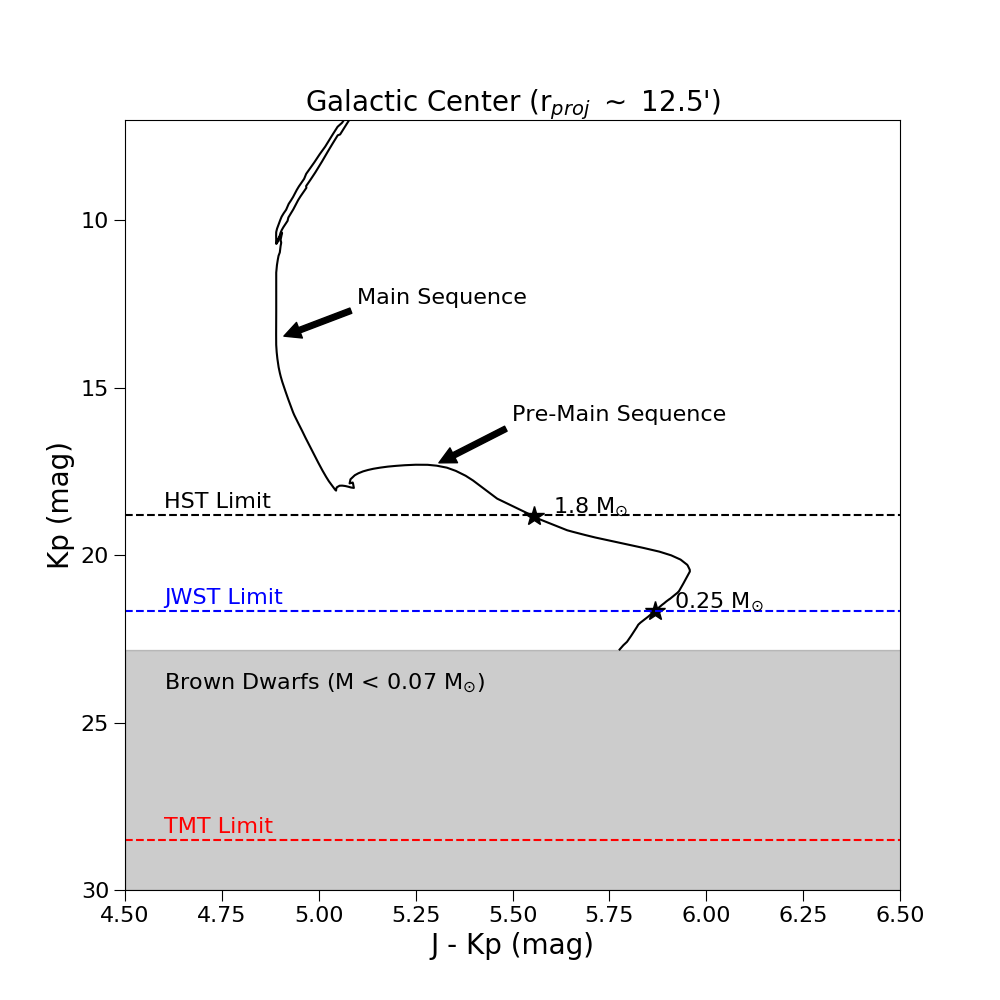
\includegraphics[scale=0.3]{TMT_comp.png}
    \caption{{\bf Left:} Model Kp-band luminosity function for the Young Nuclear Cluster showing the relative sensitivity of Keck spectroscopy (Kp $<$ 15.5 mag) and future TMT+IRIS spectroscopy (Kp $<$ 21 mag). With US ELTs, the pre-main-sequence turn-on will be detectable at Kp$\sim$17.5 as well as the full IMF shape down to $\sim$0.4 M$_{\odot}$. Figure taken from \citet{Lu:2013}. {\bf Right:} The TMT confusion limit (red dotted line) compared to the JWST confusion limit (blue dotted line) and HST completeness limit (black dotted line) for the Arches cluster near the Galactic Center. With US ELTs, the confusion limit is not reached until well beyond the hydrogen burning limit.}
    \label{fig:TMT_YNC}
\end{figure}

%MA This is not just for the GC; similar problem arises for all clusters in the Galacticmbership disk. The IMF most likely turns over but the field LF keeps rising at fainter magnitudes. Below ~0.2Msun the contamination is higher than cluster members for a lot of the cluster regions. 

{\bf \large The Initial-Final Mass Relation}

One of the most influential periods in a stars' life is actually its death, where it spreads heavy elements and injects energy, sometimes violently through supernovae, into its surrounding. The impact of a star's death is closely tied to its mass and we do not have a clear mapping between the initial mass of a star, how it dies, and the type and mass of compact object that results (Figure \ref{fig:ifmr_theory}). Mapping this initial-final mass relation is challenging simply because black holes and neutron stars are very difficult to find.  
 
\begin{figure}
    \centering
    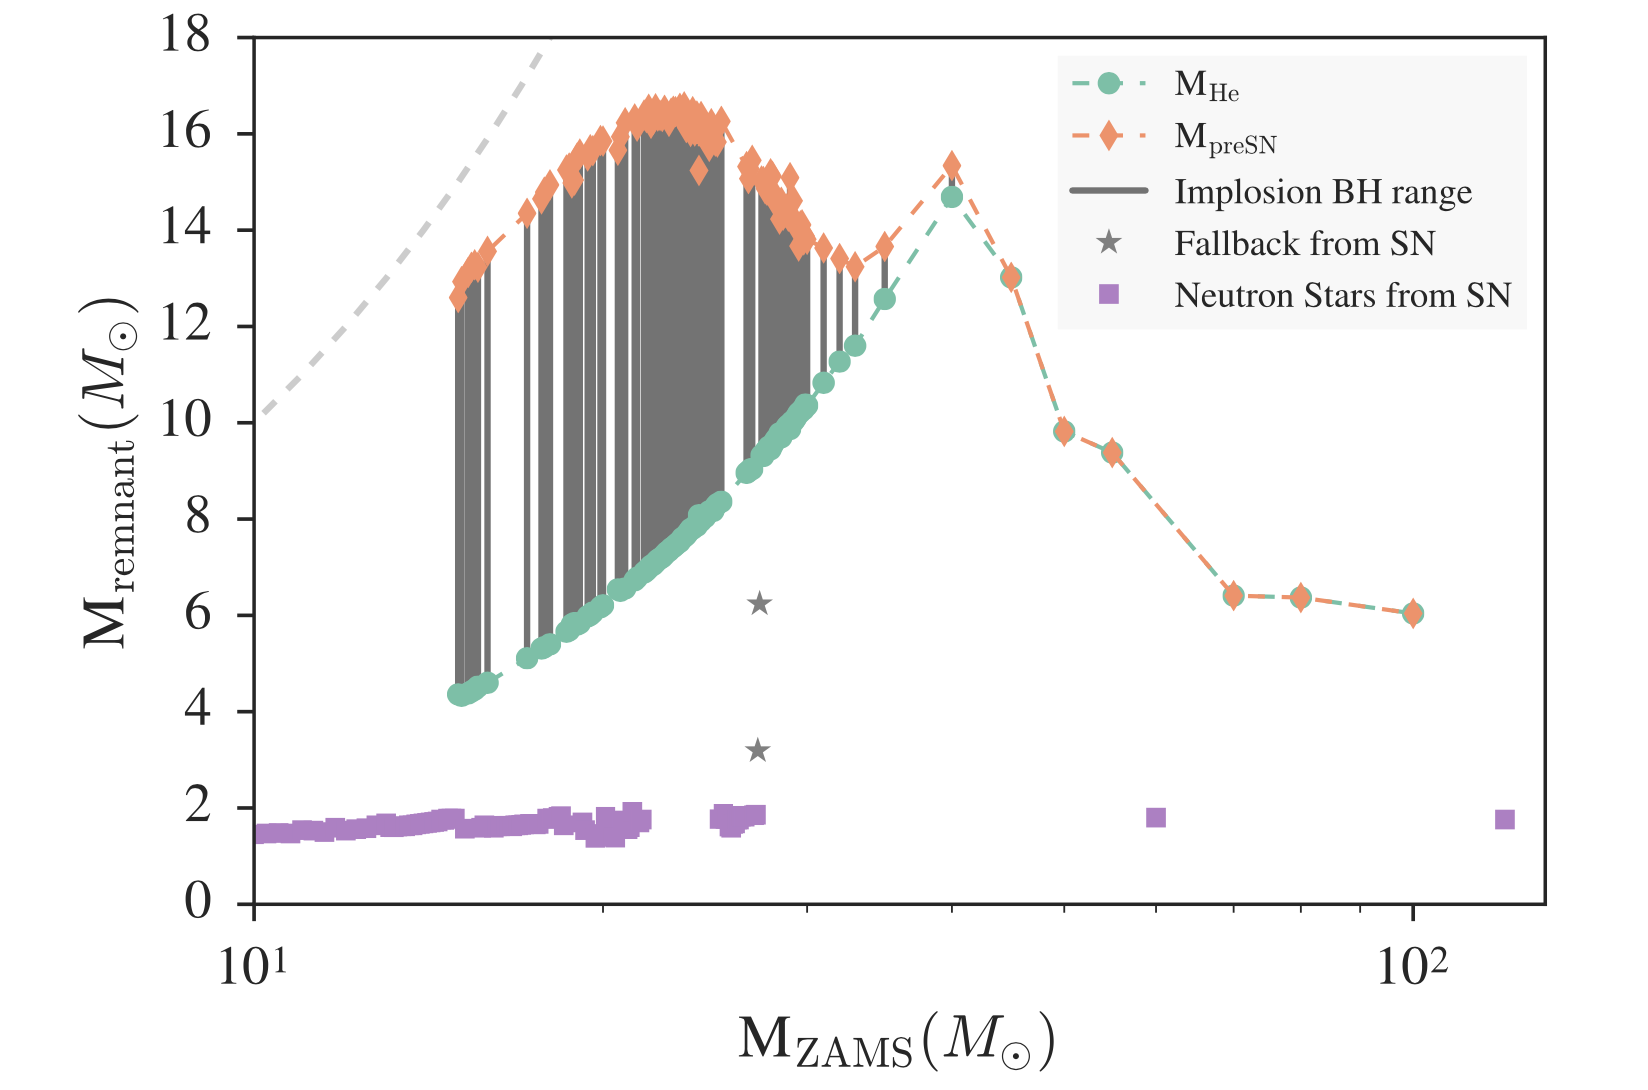
\includegraphics[scale=0.4]{IFMR_raithel.png}
    \caption{Only in the last 2 years have simulations of supernovae begun to predict a quantitative initial-final mass relation (IFMR). Current predictions produce a probabilistic relationship between the initial stellar mass and the final black hole or neutron star mass. Figure reproduced from \citep{Raithel:2018}.
    \label{fig:ifmr_theory}
    }
\end{figure}

A novel approach to detecting low-luminosity objects such as black holes and neutron stars is to use gravitational microlensing. Black holes or neutron stars that gravitationally lens background stars produce a photometric magnification that has a long duration ($>$1 months). However, a chance alignment of two slow-moving normal stars has a similar photometric signal. Fortunately, dark lenses also induce an astrometric shift in the apparent position of the background star that can be $>$0.3 mas. This astrometric shift scales as $\sqrt(M_{\textrm{lens}})$ and, if measured, it allows you to weigh dark lenses.

Only the combination of photometry and astrometry can be used to estimate the mass of the lens and determine if it is indeed a compact object. Fortunately, there is an abundance of wide-field photometric surveys planned for the next 10-20 years, including LSST and WFIRST, that will increase the number of dark lens candidates by a factor of 10-100. Current telescopes lack the astrometric precision to measure the masses for this large number of candidates and find the black holes and neutron stars. The US-ELTs are ideal, delivering astrometric precisions as good as 15 $\mu$as on faint stars even in crowded regions where Gaia, HST, and JWST, are insufficient. Thus, when a candidate dark lens is identified in a photometric survey, one of the US-ELTs can be triggered within a few days to observe the astrometric signal and get the lens mass. Also, the $\times$15 mas resolution of the US-ELTs will allow us to further confirm dark lenses after they move away from the background star in just a few years.

\begin{figure}
    \centering
    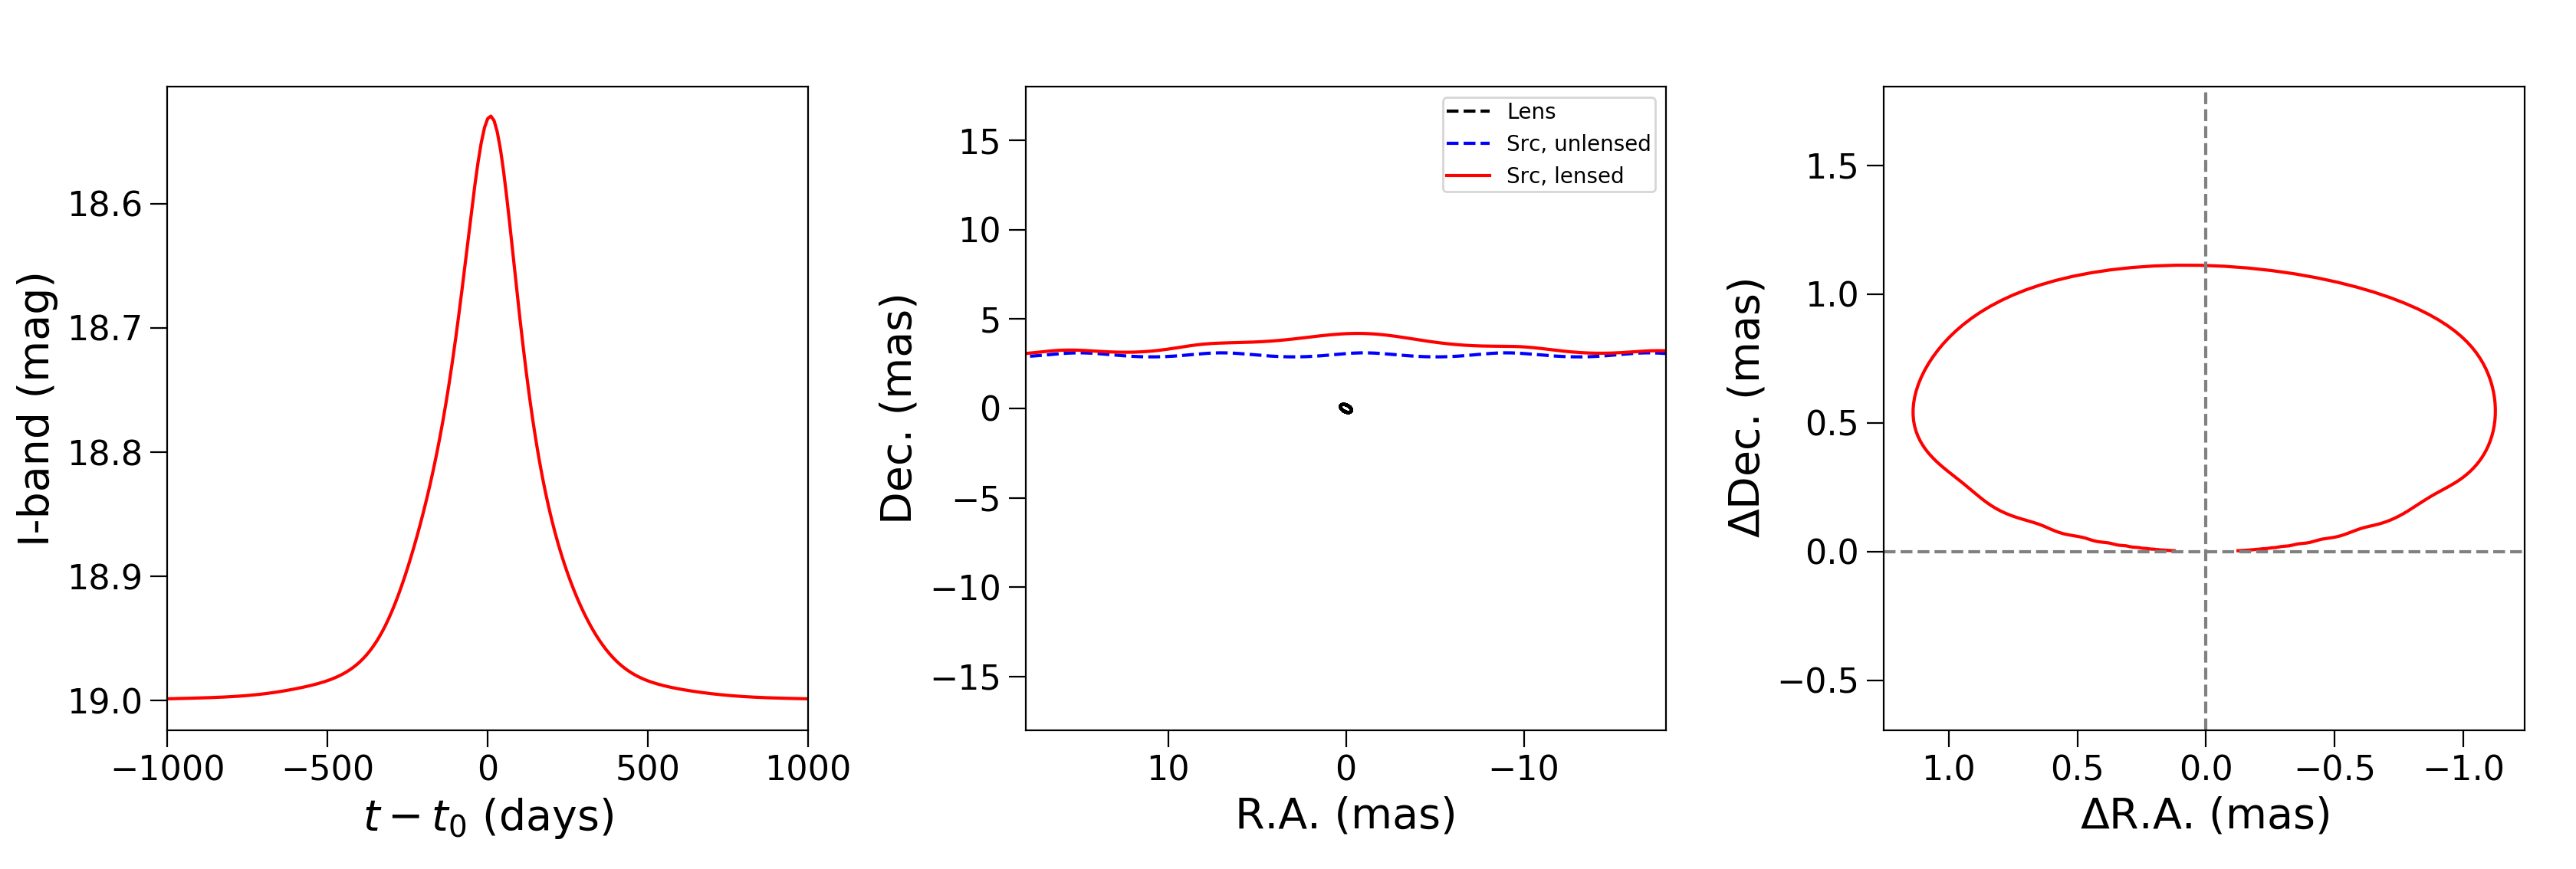
\includegraphics[scale=0.27]{phot_astrom.png}
    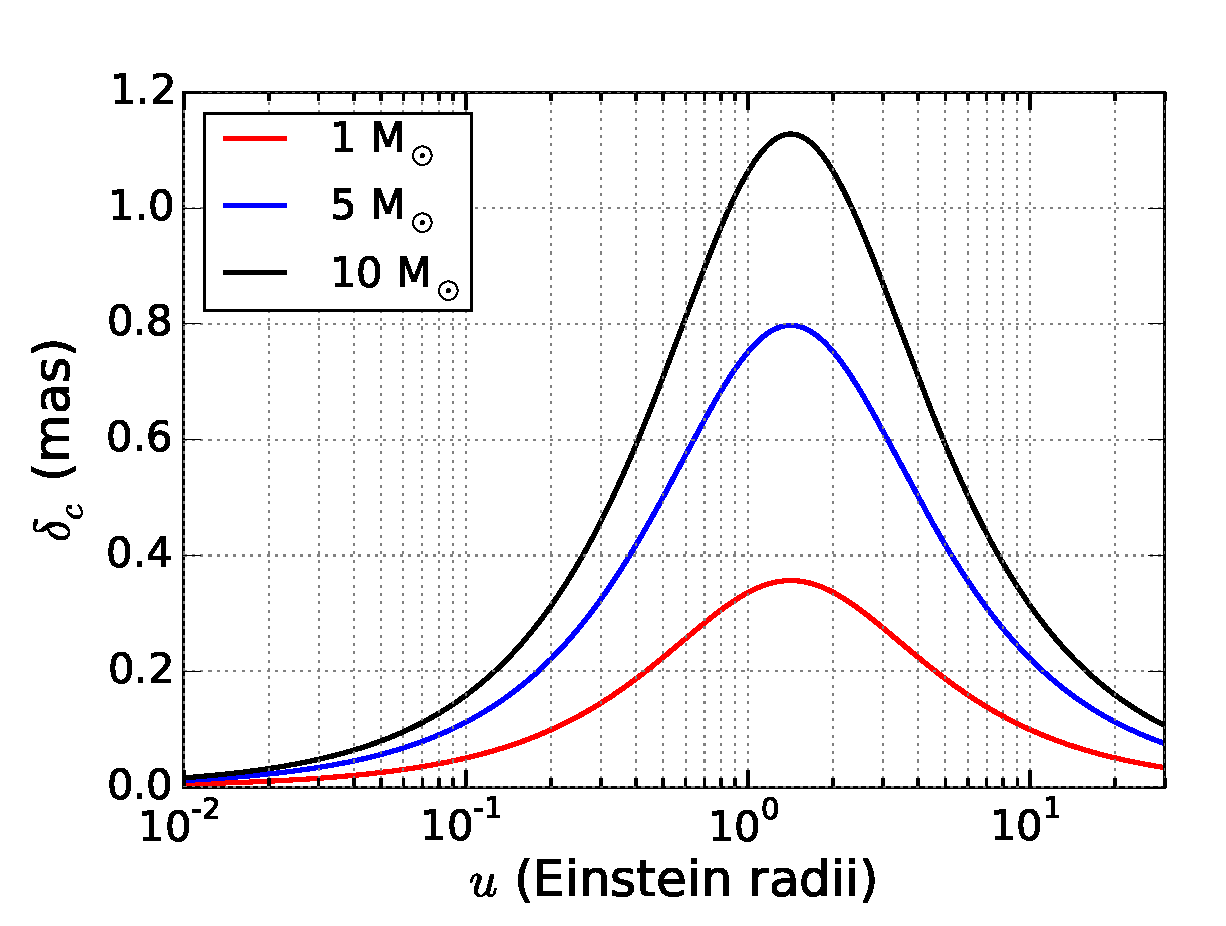
\includegraphics[scale=0.22]{MassTrend.pdf}
    \caption{Photometry and astrometry for a black hole at 3 kpc lensing a background star at 6 kpc and a relative proper motion of 8 mas yr$^{−1}$. {\em Left:} Photometric light-curve. {\em Center left:} Astrometry of the lens and source, including parallax, as would be seen on the sky. {\em Center right:} Astrometry of the source after the proper motion is removed. {\em Right:} Astrometric lensing signal vs. separation (or time) for different mass lenses.}
    \label{fig:astrom_lens}
\end{figure}

TO DO: Understanding LIGO BH-BH mergers, find the binary black holes (before merging), primordial black holes. 

% \textbf{Candidate discovery with all-sky surveys (ZTF, LSST)}
% Astrometric microlensing is an expensive measurement and must be undertaken only on those targets already known to be undergoing a microlensing event. Photometric microlensing, or the temporary achromatic amplification of a star’s brightness, is an inexpensive measurement that can be searched for on millions of stars per night. Microlensing surveys to date have focused on observing regions of high stellar density (galactic center, small and large magellanic clouds) to maximize the probability of detecting microlensing events. The next generation of all-sky surveys present the first opportunities to search for microlensing events throughout the galaxy and place meaningful constraints on the nature of gravitational lenses at various galactic latitudes.  The Zwicky Transient Facility (ZTF), a new telescope largely funded through the National Science Foundation's Mid-Scale Innovations Program (MSIP), will generate petabytes of data while conducting a public galactic plane survey in both g and R band filters. These observations strike a balance between areas of the sky with high stellar densities and exploring galactic latitudes not yet observed for microlensing to date. ZTF will generate a near real-time alert stream populated with potential transient candidates found on difference images generated by the telescope. The Large Synoptic Survey Telescope (LSST) will produce an alert stream to the public using the same infrastructure, with an observation cadence and footprint still yet to be determined. Innovative software stacks for extracting valuable science from these alert stream architectures will aid in the discovery of microlensing events for years to come.

% \textbf{WFIRST}
% Once WFIRST launches, we will move from a regime of detecting 10s of black hole lensing events each year to NNNN events per year. This will dramatically increase the sample of BH lenses with very precise multi-band photometry and simultaneous astrometry. However, WFIRST doesn’t provide continuous coverage of long-duration events because only 40\% of the mission is focused on the microlensing survey and the Galactic Bulge will only be covered for a few months out of the year. The long-duration BH lensing events will likely have incomplete coverage as a result. The next generation of large ground-based telescopes (e.g. TMT and GMT) equipped with adaptive optics systems can provide targeted follow-up during WFIRST gaps. Furthermore, WFIRST is at an L2 orbital position (CHECK) so combining TMT with WFIRST observations will allow us to measure the space-based microlensing parallax that can be combined with the astrometry and photometry to measure the distances to both the lens and source. This will finally allow us to constrain every single parameter for a lensing event, independent of any Galactic model assumption, for a large sample of BH and other compact object lensing events.  Finally, the large ground-based telescopes can provide astrometric measurements for the lowest mass compact objects that WFIRST can’t measure (e.g white dwarfs).  White dwarfs observed today with masses are mostly luminous, more massive, closer, solar metallcity? Can we probe some fainter, lower mass white dwarfs thare of interest? Is that interesting??? 
% Also measure their kick velocities, binarity.

% \begin{figure}
%     \centering
%     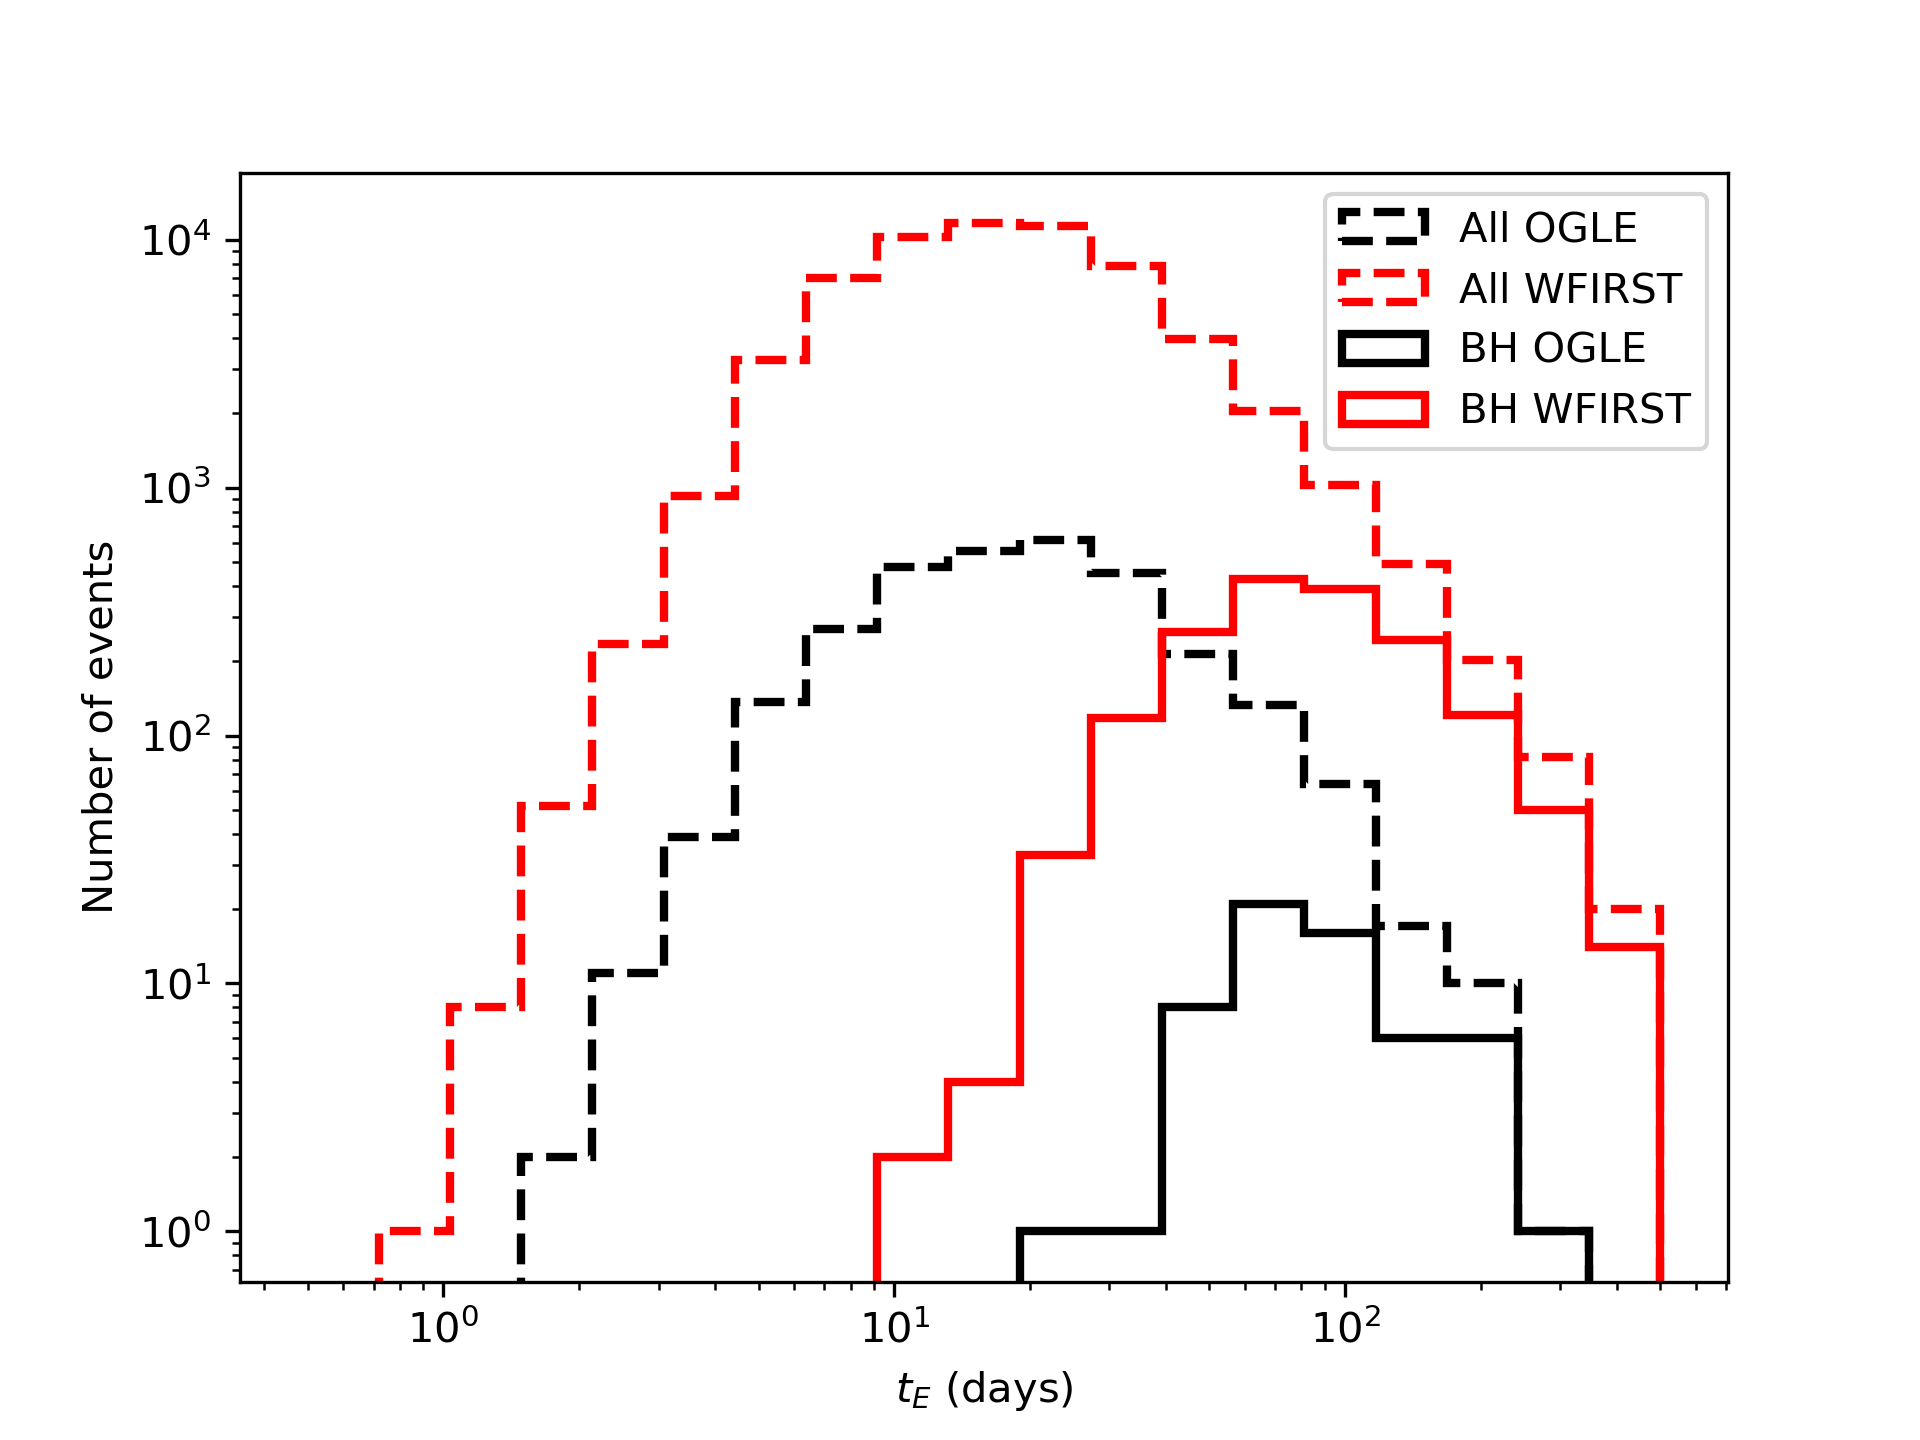
\includegraphics[scale=0.5]{wfirst_v_ogle.png}
%     \caption{Number of events seen, WFIRST vs. OGLE. WFIRST will see around 20 times more events overall, and 27 times more BH events than OGLE. The scaling on the y-axis is arbitrary-- identical areas were surveyed for identical durations and with identical cadences ( 4 x 0.34 square degree patches, for 1000 days, at a cadence of 100 days.) The differences are 1) the seeing disks (0.5'' for OGLE, 0.085'' for WFIRST), 2) limiting magnitude (I $< 22$ for OGLE, H $< 26$ for WFIRST). Both of these are constrained to have fblend $>$ 0.1 in their respsective photometric bands, with u0 $<$ 2.}
% \end{figure}

% \textbf{Search for primordial black holes (this is a tangent)}

% TELESCOPES AND INSTRUMENTS
%
% Discuss the program requirements for the telescope(s) (GMT and/or TMT), instrumentation, 
% and adaptive optics systems.  Use of both TMT and GMT in an integrative fashion merits 
% particular attention.  If the program can be carried out using instruments planned for the 
% GMT/TMT early-light suites, discuss what particular capabilities (e.g., spectral resolution, 
% angular resolution, AO performance, etc.) are required.  If new capabilities beyond the 
% defined early-light instruments are needed, describe the requirements in a suitable level 
% of detail.

\telinstreq

\noindent
{\bf IMF:}
In order to measure the IMF, both photometry and spectroscopy is required: stellar masses are extracted from multi-band photometry at all magnitudes and spectroscopy is needed to constrain the luminosity distance and calibrate the mass-luminosity relationship in each cluster.
Confusion with the surrounding field populations is a major limitation that can be overcome by using precise proper motions to select cluster members (Figure \ref{fig:Arches_cmd}). 
For both types of observations, TMT/IRIS and GMTIFS will be the workhorse instruments, using the imager for the high-precision astrometry and the IFU for the spectroscopy.
The ability to obtain this observations in both hemispheres significantly increases the number of targets that can be targeted and thus the range of environments that can be probed. 
In addition, GMTNIRS will be valuable to provide high-resolution spectroscopy for individual objects of particular interest, such as multiplicity monitoring for very low mass stars as well as studying the properties of circumstellar disks in the young stellar populations.

 
 \begin{figure}
    \centering
    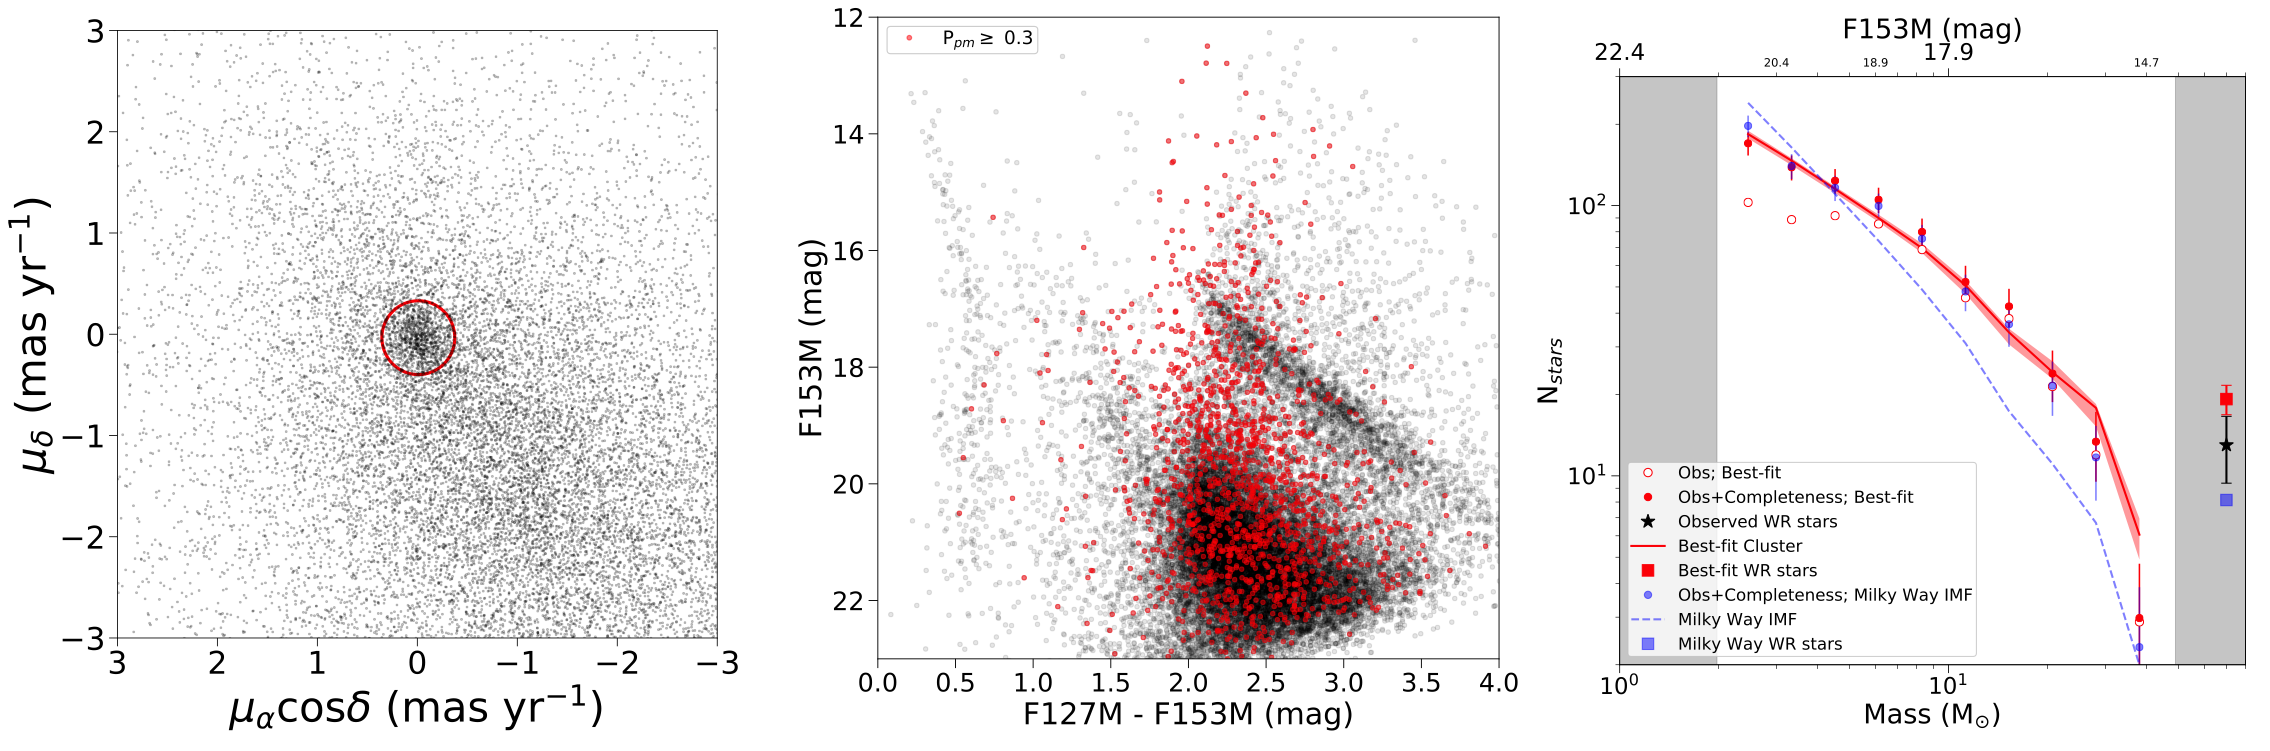
\includegraphics[scale=0.4]{Arches_IMF_3panel.png}
    \caption{Proper motions are a critical tool for eliminating field contamination when measuring the IMF of star clusters. {\bf Left:} A vector point diagram of the stars near the Arches cluster. Stars bound to the cluster have similar proper motions and thus form a well-defined clump in this space (red circle), from which cluster membership can be determined. {\bf Middle:} The color-magnitude diagram of the Arches field, with cluster member candidates highlighted in red. Note that there is significant overlap between the cluster and field star populations, causing significant contamination without proper-motion selection. {\bf Right:} The IMF of the Arches cluster (observations as red points, best-fit model as red shaded region) measured to down to 1.8 M$_{\odot}$ \citep{Hosek:2018b}. The cluster is found to have an systematic overabundance of high-mass stars relative to the IMF of nearby star forming regions (blue dotted line). WIth ELTs, we will extend the IMF to the brown dwarf regime, providing key constraints for star formation theory.}
    \label{fig:Arches_cmd}
\end{figure}
 
%Proper motions are a valuable tool for identifying members of stellar clusters. The Young Nuclear cluster at the Galactic Center is incredibly limited by crowding, but a characterization of its stellar population is necessary to explain its anomalous age and constrain its formation scenario. In addition, recent NIR proper motion studies of the Arches cluster have assessed proper motion cluster membership for stars down to $\sim$2.0 solar masses outside of the cluster core (Figure \ref{fig:Arches_cmd}), but the production of a complete proper motion catalog in the cluster core is currently limited by crowding. ELTs’ higher spatial resolution will (1) mitigate the effect of crowding on stellar completeness and (2) provide higher-fidelity proper motions of clusters in the massive core. This allows us to sample the cores of dense, young massive clusters which are differentiated from the extended cluster population photometrically (i.e., by mass segregation) and dynamically. 
		
{\bf IFMR:} The regions that are most suitable for lensing studies of compact objects created during the death of a star are towards the Milky Way Bulge, which is visible both from the Northern and Southern hemispheres. 
Searches for primordial black holes or black holes born from Pop III stars is towards M31 (North) and the LMC/SMC (South). Coverage of both hemispheres is essential. This case requires high-precision astrometry and high spatial resolution. TMT has the advantage here with a larger aperture and also the gravity-invariant IRIS imager. However, many BHs and neutron stars may be in binary systems, which can affect the mass measurement, and high-resolution spectroscopy (R$\sim$50,000) at the diffraction limit of the US-ELTs, as is available on GMTNIRS, can easily detect the binary from orbital motion. 

% EXPERIMENTAL DESIGN
%
% Describe the details of the observational program, including:
%  o Target/sample selection.  This may be a description of a target selection strategy that would be
%    appropriate in the future when the project would be executed. Specific targets may be specified,
%    particularly if they demonstrate the value of a 2-telescope, 2-hemisphere system.
%  o A description of the required observations.
%  o Signal-to-noise requirements and exposure time estimates.  Because the detailed parameters of future
%    instruments may not be precisely known now, this section should discuss the assumptions adopted.
%  o Special requirements for observing conditions (if appropriate), in particular with regard to
%    image quality and adaptive optics, precipitable water vapor, or other special conditions.
%  o Scheduling requirements (as appropriate), including lunar phase, observing cadence,
%    and/or timing constraints.
\expdesign

\noindent
{\bf IMF:} 
The IMF analysis will require both imaging and spectroscopy. Astrometric observations will need to be obtained in a single filter for at least 3 epochs over a two year baseline in order to obtain proper motions. Photometry in at least one additional filter is required for color and extinction information. Additional spectroscopy of a subset of cluster candidates will be required to calibrate the mass-luminosity relationship and quantify field contamination within the sample. Because of the high-density of many of these clusters, adaptive optics will be required to overcome stellar crowding.

\underline{Targets:} 
%mwhosek: I wasn't sure what clusters corresponded to those referred to in the observing program summary. Here are a few guesses
Milky Way: Orion Nuclear Cluster, Arches Cluster, Quintuplet Cluster, Young Nuclear Cluster, Westerlund 1, Westerlund 2 (what about low-mass regions? As I mentioned above they are quite different observing wise and it would probably confuse this proposal to include them. NGC3603 is not on the list?)
LMC: R136 
SMC: N90? 

As these targets are spread among both the Northern and Southern hemispheres, both ELTs are needed in order to achieve this science. 

\underline{SNR requirements:}
The astrometric observations require a minimim SNR of 16 in order to obtain proper motions at sufficient precision to calculate accurate cluster membership probabilities. Additional photometric measurements in other filters for color information require a minimum SNR of 5. 
){\bf SNR of 5 per filter will give some 30\% uncertainty in color which is way too much for dereddening. SNR of 16-20 for all measurements seem reasonable})
%mwhosek: Spectroscopic requirements are tricky because they will change with spectral type, resolution, and wavelength range. We needed at least SNR=50 for O-type stars at K-band and R = 4000, maybe that is enough to start? I'd imagine we might need simulations to put this on firmer ground.

{\bf IFMR:}



% OBSERVING PROGRAM SUMMARY
%
% Summarize the overall observing program.  This should include:
%  o A high-level review of the program as it would be executed, potentially over several years,
%    including the sequence of observations if relevant.
%  o The total observing time required for each telescope, instrument, and instrument mode used,
%    based on the detailed information from the Experimental Design.

\obssum

\noindent
{\bf IMF:}
We will target $\sim$6 clusters in the Milky Way, 4 clusters in the LMC and SMC {\bf number of clusters should be the same as in the target section}, $\sim$4 clusters in M82, and 3 dwarf galaxies. Each cluster requires deep imaging (2-5 hours) in multiple bands and the imaging in one filter is repeated three times, once per year. Multiple epochs will be crucial in separating field and cluster stars for the Galactic clusters. However, even after selecting members based on proper motion there will be some contamination. Spectroscopy of a subset of the candidates will be used to quantify and hence correct the field contamination. The dwarf galaxies will likely require 6-6 pointings each to build up the sample of stars. The clusters in M82 and the LMC/SMC will require IFU or MOS spectroscopy to calibrate the mass-luminosity relationship. 
We estimate this program would require ~140 hours spread over 3-5 years to comprehensively measure the IMF in a broad range of environments.

{\bf IFMR:}
The astrometric microlensing experiment requires IRIS or GMTIFS AO-fed imaging and high-precision astrometry. GMTNIRS R$\sim$50,000 spectroscopy will be used to follow up any binary microlensing events. 
Targets selected from WFIRST will typically be H=20 and we will need high SNR to reach the needed astrometric precision. 
Typical exposures times will be $\sim$5-10 minutes of exposure time per epoch per target and we need $\sim$100 targets repeated 10 times each (i.e. 1,000 $\times$10 min) over 4-5 years to build up a sufficient sample of black hole and neutron star masses. We estimate this program requires ~160 hours spread over 5 years to comprehensively measure the intial-final mass relation, binarity, and kick velocity distribution for black holes and neutron stars.



% LEGACY VALUE
%
% Discuss the legacy value of these observations and the data they would generate for the broader 
% scientific community, including a description of potential data products and the ancillary 
% science that might be enabled by this dataset.

\legacyvalue
\noindent
{\bf IMF: } The IMF aspect of this program will produce a star catalog for each of the target clusters, containing photometry, proper motions, stellar mass, and proper-motion based cluster membership probabilities. Spectroscopic measurements will be obtained for a subset of the catalog as well. There is a large amount of ancillary science that can be done with such data, including:

\begin{itemize}
    \item Star Cluster Evolution: ELTs' can probe clusters at their earliest time and thus the initial stellar distribution; mass segregation, testing whether it is primordial or dynamical, and as an important effect for cluster evolution; high-quality radial and velocity disperion profiles, which reveal the current dynamical state of a cluster
    \item Circumstellar Disk Evolution: Circumstellar disks can be detected via infrared excess around probable cluster members, allowing for study of disk evolution as a function of stellar mass, environment within a cluster, and across different clusters with different properties (total mass, metallicity, density, etc)
    \item Stellar Evolution: The high-quality cluster samples with photometric and spectroscopic information over a wide stellar mass range and at different ages provide strong constraints for stellar evolution and atmosphere models
\end{itemize}

%ELTs’ can probe clusters at their earliest time and thus the initial stellar distribution 
%Mass segregation. Largely a spatial resolution issue hence ELT science - 
%The magnitude of mass segregation in star clusters is an important measure that constraints their dynamical evolution histories. To obtain precise mass profiles, high-resolution imaging is required that can handle high crowding and detect low-luminosity stars at the central region of massive clusters.

% \textbf{Integrated Light Spectroscopy}
% Key: integrated light from nearby galaxies (this is hard)

%Ancillary science enabled by this program is the exploration of circumstellar disks for the young clusters in our sample, both as a function of mass within a single cluster and as a function of environment across different clusters, as well as the calibration of stellar evolution models to very low masses across different metallicities.

%%% OTHER ANCILLARY SCIENCE
% Cluster dynamical evolution (e.g. mass segregation, core collapse
% Star formation simulations: feedback physics
% Tests of stellar evolution models

%\textbf{Star Formation Simulations}
%Key: larger clusters, more feedback physics, match environments to observed clusters.

%\textbf{Stellar Evolution Models: }
%Essential for converting observed properties into masses
%ELT can cross-match spectroscopic, photometric, and astrometric observations, allowing for a check on current stellar evolution models and isolated techniques used on previous datasets, eg: matching theoretical isochrone models to photometric analysis of HST data that are lacking spectroscopic confirmation. ELT will constrain photometrically valid models that can then be used on spectroscopically incomplete datasets.


%\textbf{Dwarf Galaxies:}
%One of the extreme environments where IMF variations have been marginally detected is in ultra-faint dwarf galaxies around the Milky Way. One of the limitations in current observations is unresolved background galaxies that overwhelmingly contaminate stellar sources, especially at the lowest masses.  The ELTs increased spatial resolution will completely eliminate issues with star-galaxy separation, allowing IMFs to be estimated all the way down to the hydrogen limit for dozens of ultra-faints (REF Gennaro+ 2018a, 2018b). TO DO: Need to know the distribution of galaxy sizes vs. magnitude... ho w

%This also has relevance for understanding the host galaxies of LIGO/Virgo sources \citep{2017ApJ...850L...4C}.

%In Figure 2, we present a preliminary analysis of how an important nearby star forming region (the Trapezium cluster in the Orion Nebula) would look through AO-assisted imaging on a 6.5 meter telescope (like Magellan) as a function of distance.  
%With their 24-30 meter diameter, the ELTs will enable resolution demonstrated [CAN WE GENERALIZE TO TMT+GMT?] below at 25 kpc on a 6.5 meter, but out to 100 kpc!  
%Such an observation would be sky background limited at physical radii $>$ 2.5 $\times$ that of the star cluster core, enabling direct star counts to measure the IMF down to the hydrogen burning limit in local group galaxies. 
%Star formation in the Galactic Center as well as the 
%sub-solar metallicity 
%LMC and SMC would be dissected with ease. 
%The ELTs will also be able to study stellar multiplicity out to several kpc, including several regions of massive star formation.  
%MA extend current studies of the ONC out to several kpc? We will still not get that many close binaries at 2kpc
%This will represent a fundamental step in understanding massive star binary properties informing models of core-collapse super nova. 
%Recent observations of the R136, a crucial analogue for forming super-star clusters in interacting galaxies, with the SPHERE extreme adaptive optics system on the ESO VLT remain confusion limited in the core (Khorrami et al. 2017 in press - https://arxiv.org/abs/1703.02876). 
%Resolving the cores of rich star clusters in the Milky Way and beyond will inform cluster evolution studies and models of black hole formation in their cores for comparison with future gravity wave detections.  
%JWST will not help here given its small aperture size. 
%To push our understanding of star formation and the IMF to extreme environments where we can hope to put all viable theories to the most stringent tests, requires the angular resolution of the ELTs to overcome the confusion limit. 

We also note that these astrometric data sets will become more valuable with time, as they can be combined with future observations to extend the time baseline and increase the precision of the proper motion measurements.

However, the objects proposed observed here further serve as references themselves; Objects like NGC3603, 30 Doradus and its central cluster R136 are used as templates for the high-z unresolved star clusters where their properties have to be determined from their integrated properties. 

{\bf IFMR: }


% ANALYSIS PLAN
%
% Describe the program requirements for data analysis and interpretation.  This may include:
%  o Data management and software needed for data reduction and analysis.
%  o Simulations needed to interpret the data.
%  o Other resources (e.g., computational, user support) that may be necessary.

\analysisplan
{\bf IMF: } Although the observations possible with the TNT and GMT are transformative for the field of IMF studies many of the tools necessary to optimize the scientific return have been developed on HST and 8 meter class telescope. 
These include software routines for details photometry and source extraction in crowded fields (
To extract astrometric and photometric measurements, a software package like Starfinder will be required, but with the ability to handle a spatially-varying PSF. These include e.g. starfinder and modified versions of daophot. 
The similar packages are used to make detailed assessment of the effects of sensitivity and crowding which are crucial to know in detail to derive the low-mass end of the IMF. 
Using state of the art stellar evolutionary models that take the pre-main sequence phase into account the near-infrared photometry will be converted into mass and age estimates. However, with the increased sensitivity we expect to obtain spectra of objects in the pre-main sequence phase using these in conjunction with the photometry to constrain the parameters for the whole photometric population. 

Spectral classification will be performed using both model spectra but also using  references from nearby star forming regions where the depth we expect to reach with the TMT and GMT have been reached already now due to the smaller distance. 
This will allow detailed relative studies between the star forming regions since the relative ages and hence masses will be well determined. 

Field star contamination will be quantified through a combination of control fields and proper motion analysis. The highly accurate proper motion expected over several epochs will provide clean color-magnitude diagrams which will further be vetted using the spectroscopic samples. 
% mwhosek: PSF-reconstruction on the adaptive optics? Not sure what the predicted astrometric precisions are without PSF-R.


{\bf IFMR: }

% SYNERGY WITH OTHER FACILITIES OR RESOURCES
%
% If relevant, describe how the proposed TMT/GMT observations complement data from other facilities. 
% This may include:
%  o Required coordination between the proposed GMT/TMT program and observations or data resources
%    from other facilities in space or on the ground.
%  o Preparatory or ancillary datasets that will be required to carry out this Key Science Program.

\otherfacilities

The US-ELTs and upcoming (near-) IR space telescopes such as JWST and WFIRST will directly inherit the growing synergy between ground and space based facilities from their immediate predecessors, e.g., Keck and HST. For IMF studies, the diffraction-limited imaging with the large collecting area of the US-ELTs will play a great role in resolving stars at the most crowded regions such the cluster core. The rest of the cluster will be covered by the space telescopes with a wider field of view, which enables constructing the IMF of the stellar system as a whole.


%%%%%%%%%%%%%%%%%%%%%%%%%%%%%%%%%%%%%%%%%%%%%%%%%%%%%%%%%%%%%%%%%%
\bibliography{imf_ifmr}
% Please do not modify or delete this line.
\end{document}

%%%%%%%%%%%%%%%%%%%%%%%%%%%%%%%%%%%%%%%%%%%%%%%%%%%%%%%%%%%%%%%%%%
